\documentclass[journal]{IEEEtran}
\usepackage{blindtext}
\usepackage{graphicx}
\usepackage[justification=centering]{caption}


\usepackage{listings}
\usepackage{color}
\usepackage{soul}

\definecolor{lightgray}{rgb}{.9,.9,.9}
\definecolor{darkgray}{rgb}{.4,.4,.4}
\definecolor{purple}{rgb}{0.65, 0.12, 0.82}

\lstdefinelanguage{JavaScript}{
  keywords={typeof, new, true, false, catch, function, return, null, catch, switch, var, if, in, while, do, else, case, break},
  keywordstyle=\color{blue}\bfseries,
  ndkeywords={class, export, boolean, throw, implements, import, this},
  ndkeywordstyle=\color{darkgray}\bfseries,
  identifierstyle=\color{black},
  sensitive=false,
  comment=[l]{//},
  morecomment=[s]{/*}{*/},
  commentstyle=\color{purple}\ttfamily,
  stringstyle=\color{red}\ttfamily,
  morestring=[b]',
  morestring=[b]"
}

\lstset{
   language=JavaScript,
   backgroundcolor=\color{lightgray},
   extendedchars=true,
   basicstyle=\footnotesize\ttfamily,
   showstringspaces=false,
   showspaces=false,
   numberstyle=\footnotesize,
   numbersep=9pt,
   tabsize=1,
   breaklines=true,
   showtabs=false,
   captionpos=b
}


\begin{document}
\title{CS548 Term Project \emph{"Side Channel Leaks over HTTPS"}}

\author{Team 14: Antoine RONDELET (20176461), Enoch LEE (), Alexis GACEL (), Felix BOSCHE ()}
\maketitle
\IEEEpeerreviewmaketitle

\section*{Abstract}

\textbf{[TODO]}

\bigskip

\emph{Keywords: web security, side-channel leaks, network analysis, privacy}

\section{Encryption}

Introduce cryptography/cryptanalysis and the fundamental terms we have seen and studied during the semester.

Then speak about C.I.A and the foundation and objectives of encryption

\begin{figure}[h]
\centering
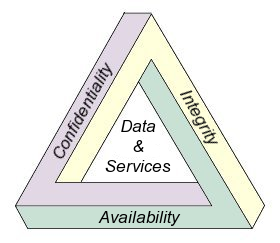
\includegraphics[width=0.37\textwidth]{images/cia.png}
\caption{The triangle of security}
\label{fig:dbBuilder}
\end{figure}

\medskip

\section{HTTPS}

\subsection{TCP/IP}
Speak a bit about TCP/IP since this is what we use for the project

\subsection{TLS/SSL}

Introduce TLS and speak about it (TLS handshake) and how it works + say that it seats between TCP and HTTP is the OSI model and so on.

\subsection{HTTP}

Introduce HTTP and present it.
IMPORTANT for our project --> say that HTTP requests are received in the same order as they are sent !



\section{Side Channel Leaks}

Present side channel leaks and previous works that exploit them to carry out attacks (timing attack on SSH, and so on)


\section{Content of our research}

\subsection{Goals}

As we said earlier in this paper, side-channel leaks have already been studied for quite a long time now. However, despite being well-known to developers, it seems that web applications are still leaking many pieces of information. While some researchers have already carried out studies on side-channel leaks on web applications, we couldn't find any paper presenting tools that automated the exploit of such information to infer the user input. Thus, we saw in this project, the opportunity to extend previous work, and build such an automated tool.

\medskip

Nonetheless, since all web application present its very own specificities, designing a tool that would work for every web application seemed to be unfeasible at first glance. That is the reason why we decided to carry our project on a chosen target web application. \\

With this in mind, our project could then be defined as building a packet-analyzing tool that could give out the user inputs by analyzing TLS traffic of the targeted web application.

\subsection{Hypothesis}

In order for us project to be successful, we decided to adopt several assumptions based on \cite{SCLeaks}:

\begin{itemize}
    \item \textbf{Successfully mounted MiTM\footnote{Man in The Middle. See more on https://en.wikipedia.org/wiki/Man-in-the-middle\_attack} attack}: This could be made possible in the case where the attacker manages to make his victim connect to a rogue wireless hotspot for instance. In such a scenario, network security technologies used on Wi-Fi wireless networks\footnote{More details: https://www.lifewire.com/what-is-wpa2-818352} do not hold, and the attacker can focus his attack on the HTTPS traffic of his victim. Note that, in our case, the attacker is passive. This means that he does not manipulate any data, but only sits between the victim and the web application, and observe the traffic.
    \item \textbf{Highly interactive target web application}: This hypothesis we make here, is a fairly weak hypothesis. Indeed, today, plenty of websites try to improve the user experience by implementing features such as auto-completion. Such functionality ensures low entropy inputs and aim to improve interactions with the user. From an attacker's point of view, such interactions between the client and server side of the web application are a bargain. They produce a lot of network traffic observable by the eavesdropper.
    \item \emph{Significant traffic distinction}: In order for our attack to be successful, the attacker should be able to differentiate two requests based on observable attributes. While, this does not mean that the attacker is able to decrypt the encrypted data, this signify that some observable attributes should provide the attacker with enough information to differentiate the network traces of different requests.
\end{itemize}


\subsection{Environment}

As aforementioned, the first part of our project has been to look for an appropriate web application to target. After a few days of research, we found that airlines website and, in a larger extent, journey websites were good candidates. In fact, they tend to offer many auto-completion features to facilitate the booking of their customers and make their experience as good as possible. Moreover, while some of them do not have protected \emph{home pages}\footnote{By protected we mean that they do not use HTTPS}, a majority of them shield their customers' activity with encrypted channels. Furthermore, we agreed in the group that customers' journey data were pretty sensitive and could help an attacker acquire valuable knowledge on his victim's habits or his location during a trip. 

\medskip

At this point, since many candidates seemed to be viable for our project, we decided to carry out our attack on the web application \emph{www.kayak.com}. This website is a fare aggregator and travel metasearch engine operated by The Priceline Group, based in the United States. Since KAYAK is available in 18 languages and used world wild, being able to achieve our attack on this website would have tremendous impact.

\medskip

Our attack has been performed on a MacBook Air running macOS Sierra version 10.12.6. However, as we will see in the next section, we needed to do a precomputation phase in order to infer the user input with some satisfiable accuracy. In order to carry out this precomputation, we used 10 machines running Ubuntu\footnote{https://www.ubuntu.com} 16.04, with 521Mb of RAM and a single core CPU.

\section{Description of the attack}

The purpose of our project was to develop a tool that would infer the user inputs on a web pages using HTTPS. In order for us to implement such a tool, and implement the inference process, we needed to build a database to confront the sniffed data size to, in order to retrieve the most probable payload it could correspond to. The idea was to test all possible entries in the search bar of the website, and observe in the meantime the network traffic we generated. If we could manage to associate our actions to our network traffic trace, then we would be able to sniff the victim's network and compare the leaked information (packet size in our case) with our own network trace, and see to which payload it corresponds.

\medskip

The following section presents the precomputation step of our attack.

\subsection{Attack precomputation}

In order to infer the victim's input, we needed to test all possible entries in the search bar of \emph{www.kayak.com}. While this could be done manually for a few payloads, this task is burdensome and error prone. In such a manipulation, the attacker has to observe his own network traffic\footnote{This can be done with software like Wireshark (https://www.wireshark.org)}, and map the request and response's packets to the payload he entered.

\medskip

Our idea was to build a set of software components dedicated to test all possible user input in the search bar of the target web application. By doing so, we could record the generated network traffic and come up with an automated way to map each payload with the corresponding network traffic. However, since we wanted to have the best "dataset" possible, to carry out our attack, we decided to iterate on this "mapping" step, and do it many times and with different machines, in order to eliminate potential noise or inconsistencies from our records.

\bigskip

\subsubsection*{The "API Caller"}

In order to ease the work of the attacker, we implemented the \emph{API Caller}, a component dedicated to test all possible input in the search bar of \emph{www.kayak.com}. This module contains a \emph{payload generator} submodule which generates all possible letter strings up to a certain length. Once all these payloads generated, they were given to the part of the \emph{API Caller} dedicated to execute requests on the target web app. \\

By examining the web application with the developer console of our browsers, we were able to know the exact URL used by KAYAK to fetch the entries of the suggestion list. Thus, we could identify the location of the user input, split the URL into different parts and include our generated payloads, as if it were the result of a "human-machine" interaction.

\begin{figure}[h]
\centering
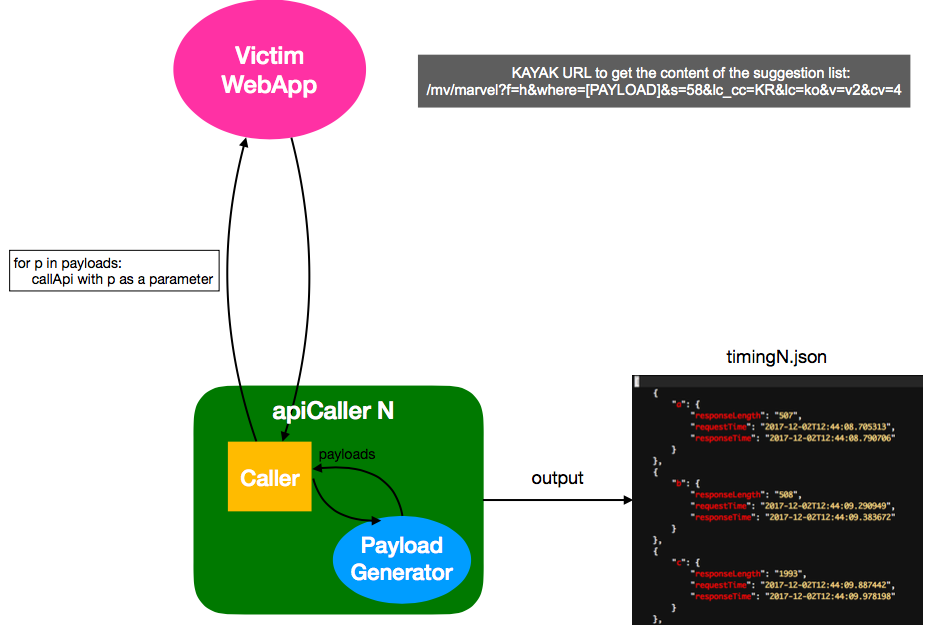
\includegraphics[width=0.48\textwidth]{images/apiCaller.png}
\caption{The apiCaller}
\label{fig:apiCaller}
\end{figure}

As shown on the figure \ref{fig:apiCaller}, the caller module receives the list of generated payloads from the generator, and sends a request to KAYAK for each payload in this list. However, in order to prevent the web server hosting KAYAK, to believe that we were DoS\footnote{Denial of Service (https://en.wikipedia.org/wiki/Denial-of-service\_attack)} attackers, we took the precaution to impose a few microseconds of sleeping time between each request. Although, this made our precomputation slower, this helped us make sure that we were mimicking actual user input.

\medskip

Furthermore, as shown on \ref{fig:apiCaller}, the output of the \emph{API Caller} is a \emph{timing.json}. This file is a JSON\footnote{https://www.json.org} array whose entries are JSON objects that associate each payload with the time the request has been made, the time the response has been received and the value of the \emph{Content-Length} HTTP header. In fact, when the attacker precomputes the database necessary to carry out the attack, the requests are initiated from his machine, and the responses are received on his machine too. Thus, at point of time, the attacker's HTTP client decrypts the traffic. Then, he can know the "real" size of the response body. Such information is always to know from an attacker's perspective and might help differentiate the victim's encrypted traffic in the next steps. \\
In addition of knowing the size of the response body, we also stored the time when we initiated the request and received the response from the server. This timing information was used to help us split the network trace. With these times, we were able to extract the packets corresponding to the sending of each payload to the server (and the corresponding requests. Indeed, since HTTP dictates that responses must arrive in the order they were requested, and since our \emph{API Caller} sends a new request after receiving the previous one, we had an ordered and easy-to-analyze network trace. Using the request and response time allowed us to know exactly which TCP traffic was generated after the request and response corresponding to a specific payload. As a consequence, the timing information provided as an output of the \emph{API Caller} was paramount for the rest of the precomputation.

\bigskip

\subsubsection*{The "Trace Builder Manager"}

As aforementioned, the purpose of the \emph{API Caller} was to lessen the burden of the attacker, by trying all possible inputs in the search bar of our target web application. While the requests and responses were sent and received, we needed to keep track of the network activity. This was the task of the \emph{Trace Builder Worker}. Each of these workers were bash\footnote{https://www.gnu.org/software/bash/} scripts. They launched one tcpdump\footnote{} daemon and an \emph{API Caller}. While the \emph{API Caller} was in charge of trying all possible user inputs, the tcpdump daemon recorded all the network trace in a \emph{.pcap} file.

\medskip

In order to maximize the output of our attack, we wanted to observe as many network traces as possible. That way we would be able to get rid of any noise in our dataset. This noise could come from the network itself, or just from the fact that HTTP headers can differ slightly from one connection to another. Indeed, we know that HTTP headers are within the data encapsulated in TCP packets. Thus, a different change in headers could add some noise in our dataset, in the sense that, for a given payload, requests and responses would not have the exact same byte size. Since \emph{User-Agent}, \emph{Referrer} and some other HTTP headers tend to change frequently from one machine/connection to another, it is likely that such changes can be felt in our data. In the case where 2 payloads generate a very different and distinguishable traffic, such changes would not necessarily be a problem. However, we observed in our study that some web-traffics were pretty similar for some pairs of different payloads. In this case, having only a few bytes of difference between 2 traffics related to the same payload could fool the attacker and threaten the viability of the inference.

\begin{figure}[h]
\centering
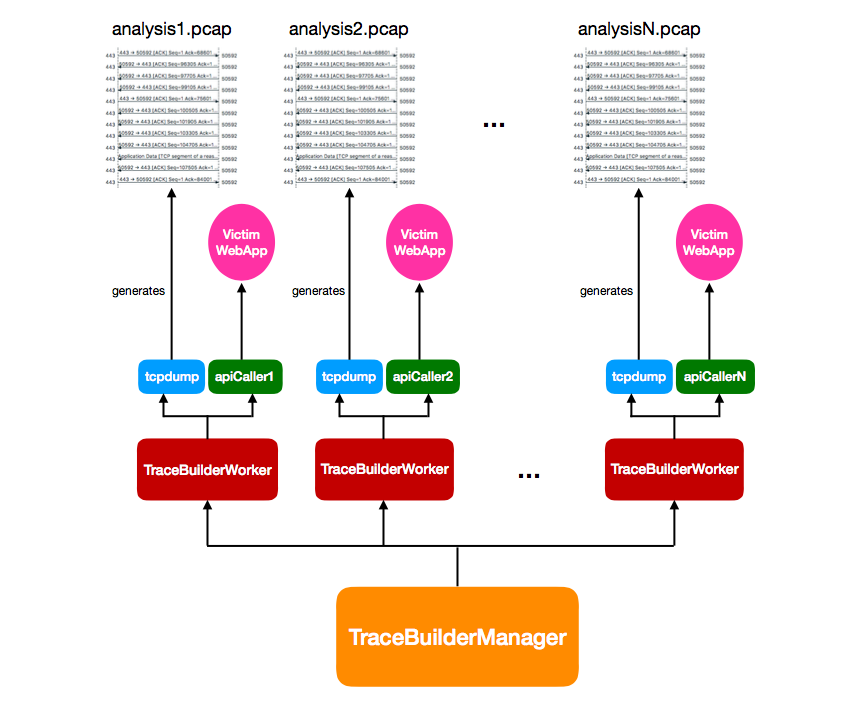
\includegraphics[width=0.48\textwidth]{images/traceBuilderManager.png}
\caption{The "TraceBuilderManager" launches many "TraceBuilderWorkers" to records multiple traffic traces}
\label{fig:traceBuilderManager}
\end{figure}

The figure \ref{fig:traceBuilderManager} shows the \emph{TraceBuilderManager}, which is the solution we came up with, in order to deal with the uncertainty described above. This component starts many \emph{TraceBuilderWorkers} which launches one \emph{tcpdump} daemon and an \emph{API Caller}. The output of  each worker is composed of 2 files: One network trace file (\emph{.pcap}) and timing file which is used to analyze the network trace as explained earlier.

\bigskip

\subsubsection*{The "dbBuilder"}

The last component involved in the precomputation step of our attack is the \emph{dbBuilder}. This module launches as many \emph{TraceAnalyzers} as the \emph{TraceBuilderManager} launched \emph{TraceBuilderWorkers}.
Each \emph{TraceAnalyzer} take the network trace file (\emph{.pcap}) and timing file generated by the \emph{TraceBuilderWorkers} at the previous step and are in charge of analyzing the network trace, and attribute to each payload tested by the \emph{API Caller}, the network traffic they generated and which was captured by the \emph{tcpdump} daemon. At the end of the analysis, each \emph{TraceAnalyzer}, outputs a \emph{resultTrace.json} file, which is a JSON file containing an array where each entry are payload mapped to the size, in bytes, of their associated request and response.

\medskip

At this point of the precomputation, one could directly begin to attack the victim. Nonetheless, as we want to remove as much noise as possible from the database, the \emph{dbBuilder} waits for each of its \emph{TraceAnalyzers} to terminate in their respective threads, and collects all the resulting \emph{resultTrace.json} files. In order for all our data to be represented in final database file, the \emph{dbBuilder} computes for each payload in the \emph{resultTrace.json} files, the mean of their request and response size. 

\begin{figure}[h]
\centering
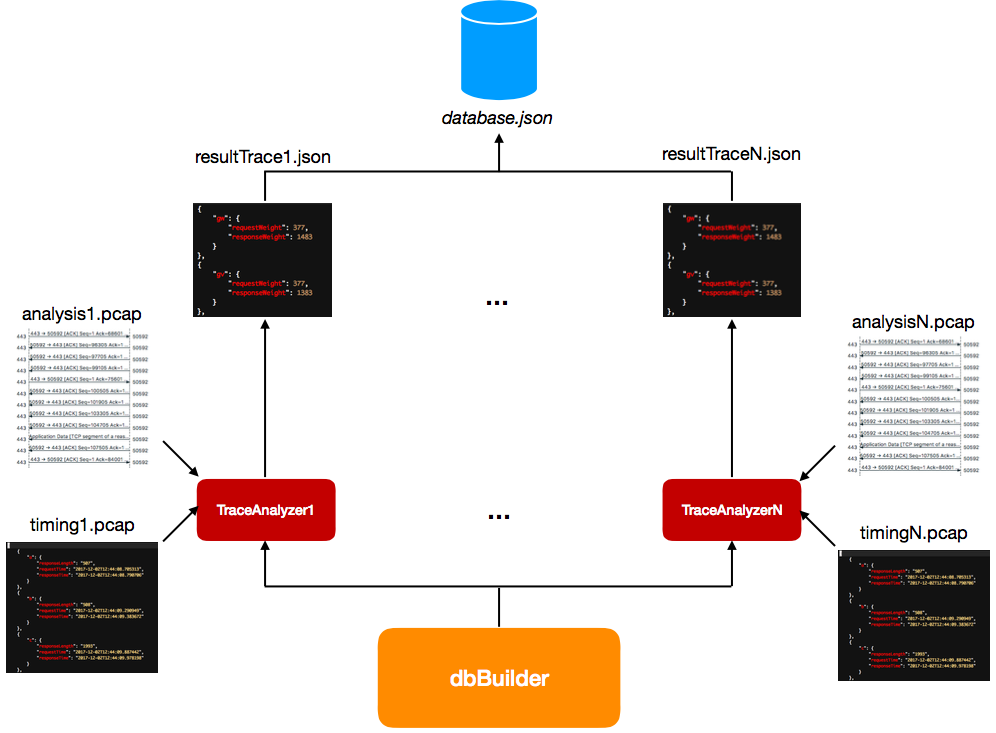
\includegraphics[width=0.48\textwidth]{images/dbBuilder.png}
\caption{The dbBuilder}
\label{fig:dbBuilder}
\end{figure}

The output of the \emph{dbBuilder} represents the end of the precomputation stage. All the steps and components mentioned in this part have been wrapped up in a bash script, \emph{attackPreComputation.sh}, which takes the number of desired network traces, the payload max length, the attacker's IP address, the target webapp's IP address and the network interface to listen/sniff on, as arguments (see figure \ref{fig:dbBuilding})

\begin{figure}[h]
\centering
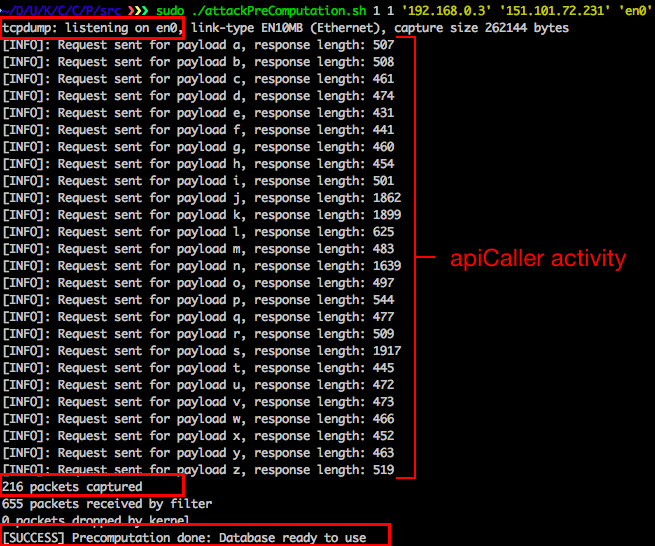
\includegraphics[width=0.48\textwidth]{images/dbBuilding.png}
\caption{The database precomputation with a single network trace and payloads of length 1}
\label{fig:dbBuilding}
\end{figure}

Now that we have talked about the precomputation, the successfully mounted MiTM attacker, should be able to carry out the attack on his victim.

\begin{lstlisting}[caption=The JSON structure of the precomputed database, label={listing:databaseStructure}]
[
	{
			"a": {
				"requestWeight": 374,
				"responseWeight": 541
			}
	},
	{
			"b": {
				"requestWeight": 374,
				"responseWeight": 548
			}
	},
    ...
]
\end{lstlisting}

\subsection{Victim's network eavesdropping}

After precomputing the database, the attacker should now be ready to eavesdrop the victim's network and infer the user's activity on the targeted web application.

\medskip

The component in charge of the attack is called: the \emph{networkAnalyzer}. This module is in charge of sniffing the victim's network traffic and analyze the data in order to return the most probable payload entered by the user. However, since we wanted to keep good performances during our attack, we don't wanted to slow down the sniffing by doing the inference on the same process. That is the reason why we split these 2 tasks in separate threads (see figure \ref{fig:networkAnalyzer})

\begin{figure}[h]
\centering
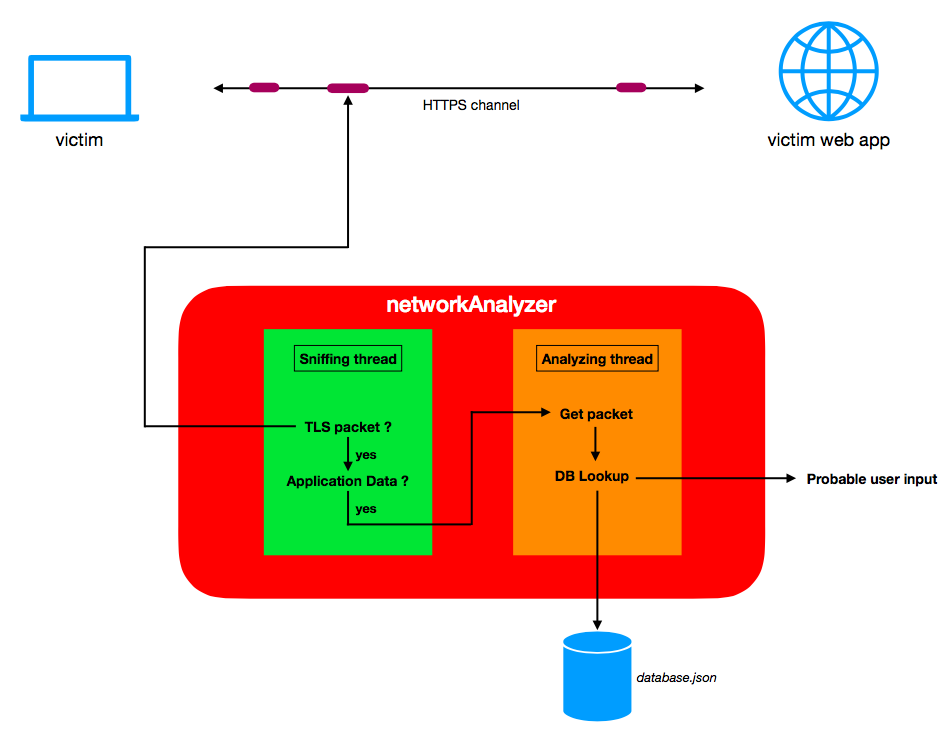
\includegraphics[width=0.48\textwidth]{images/networkAnalyzer.png}
\caption{The networkAnalyzer}
\label{fig:networkAnalyzer}
\end{figure}

\bigskip
\subsubsection*{The Sniffing thread:}
The \emph{sniffing thread} aimed to do a \emph{LiveCapture} of the victim's network and determine the nature of the captured packet (whether it is a TLS packet or a TCP ACK for instance). Once the \emph{"sniffer"} was sure that the captured packet was a TLS packet, the next step was to make sure that this packet was actually carrying application data (and not a TLS Alert or other kind of TLS messages). If these 2 conditions were met, then the packet's information were written in a queue\footnote{https://docs.python.org/2/library/queue.html} whose data was consumed by the \emph{Analyzing thread}. 

\medskip

\emph{\underline{Note:}} In order to analyze and dissect TLS and TCP packets sniffed on the network, we used the python module \emph{Pyshark}\footnote{https://kiminewt.github.io/pyshark/} that is a wrapper around Tshark (Wireshark's CLI tool). This module was pretty handy since it enabled us to access the fields of each packet pretty easily. Nevertheless, we felt that this module was pretty slow to capture live traffic. Therefore, we often sniffed a victim's packet a few seconds after it was actually emitted by the victim user. Our attack can, thus, be qualified as a "near real time attack".

\bigskip
\subsubsection*{The Analyzing thread:}

While the thread dedicated to sniff the victim's network filtered TLS packets, carrying application data, before writing them into a queue; the thread devoted to analyze the packets, consumed the data from the queue. Each object read from the queue was a python object whose attributes were a \emph{direction} and the \emph{size} of the packet in bytes. The \emph{direction} attribute specified whether the packet was sent as part of a request (client to server communication) or received as a response from the server. The \emph{size} field contained the size in bytes of the application data encapsulated in the TLS packet. \\
Based on this information, the \emph{analyzing thread} was able to do a lookup in the database and output the most probable payload. The database lookup is different is the case of requests and responses. However, in both cases, this can be split into 2 parts. Let's focus on requests first:

\begin{itemize}
\item The analyzer consumes a piece of data from the queue. The \emph{direction} attribute is set to "Request". Thus, the \emph{analyzer} only compares the value of the \emph{size} attribute to the stored payload's \emph{requestWeight} JSON field (see listing \ref{listing:databaseStructure} for the DB structure).
\item The comparison between "observed" request size and request size of values stored in the database has been implemented with a percentage of difference. The pseudo algorithm is described below:
\begin{lstlisting}[caption=Pseudo algorithm to infer user input during a Request, label={listing:inferenceRequest}]
// Step 1- Read data sent by the "sniffer"
sniffedData <- queue.get()
sniffedDataSize <- sniffedData.size
sniffedDataDirection <- sniffedData.direction

// Step 2- Find the most probable entries that match the observed Request traffic
minimumDifferencePercentage = 100
potentialPayloads = []
for each entry in the database, do:
	// Compute the percentage of difference
    absDiff <- |sniffedDataSize - entry.requestWeight|
    average <- (sniffedDataSize + entry.requestWeight) / 2
    percentageOfDiff <- (absDiff/average) * 100
    if percentageOfDiff < minimumDifferencePercentage:
    	append entry to potentialPayloads
return potentialPayloads
\end{lstlisting}
\end{itemize}

Using the percentage of difference to infer the probable user input allowed us to have more flexibility. Indeed, exact matching of request/response traffic size would not have been a good fit since we saw earlier in this paper that the actual TLS packet size, for a same payload, differed slightly from one request to another. Thus, doing exact matching would have produced very bad results in this case. Instead, we decided to measure the percentage of difference between the sniffed packets' size and the entries in our database. The result was a list of potential payloads. This list contained all the payloads for which the percentage of difference with the sniffed value was minimal. Returning such a list allowed us not to lose any information, and provide the attacker with the best information as possible.

We can see in the listing \ref{listing:inferenceRequest} that when the \emph{"analyzer"} tries to find the payload corresponding to a sniffed request packet, it does a lookup in the entire database. This lookup can hardly be avoided because when the user inputs some data in the search bar, we do not have any clue of what this data can actually be. However, in the case of a response, the situation is different. Indeed, we know that the web applications responds what the user requested. Thus, in the case of a response analysis, we can optimize the lookup in the database. Instead of iterating on the entire list of records of the database to find the payloads with the closest response sizes, we can use the fact that we already observed the user request. Since we observed the user request and returned the list of potential payloads, we already eliminated a lot of entries of our database, and narrowed down our research to a subset of all payloads. The idea is to use this subset of the database in order to find the user payload by using the information we got from the traffic of the response. \\

The pseudo code corresponding to the inference of the user payload becomes:

\begin{lstlisting}[caption=Pseudo algorithm to infer user input during a Response (using the result of the inference on the request), label={listing:inferenceResponse}]
// Step 1- Read data sent by the "sniffer"
sniffedData <- queue.get()
sniffedDataSize <- sniffedData.size
sniffedDataDirection <- sniffedData.direction
// [Response Only] We use the result of the observation of the request
potentialPayloadsFromRequestObservation

// Step 2- Find the most probable entries that match the observed Response traffic (Based on what we observed during the request)
minimumDifferencePercentage = 100
probablePayloads = []
for each entry in the potentialPayloadsFromRequestObservation, do:
	// Compute the percentage of difference
    absDiff <- |sniffedDataSize - entry.responseWeight|
    average <- (sniffedDataSize + entry.responseWeight) / 2
    percentageOfDiff <- (absDiff/average) * 100
    if percentageOfDiff < minimumDifferencePercentage:
    	append entry to probablePayloads
return probablePayloads
\end{lstlisting}

So here, we used the fact that the content of the response was tied to the content of a request, by trying to find the user input in the potential payloads returned during the analysis of the request. This made our program faster. Furthermore, since we used information from requests and responses, our program became more robust.


% Need to include the demo on the attack before the section "Results" to have the image embedded on top of the "Results" page

\begin{figure*}[h]
\centering
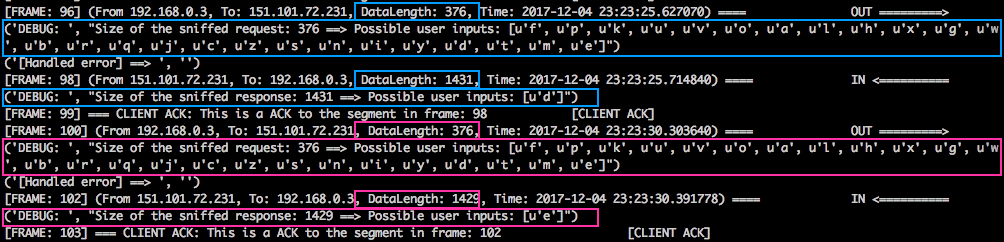
\includegraphics[width=\textwidth]{images/sniffingInference.png}
\caption{The network analyzer inferring correctly the user input over an HTTPS connection}
\label{fig:sniffingInference}
\end{figure*}

\section{Results}

Looking back to our project proposal a few weeks ago, we proposed to "Build a packet-analyzing tool that could give out the user keypresses on a highly interactive web application". After reading some papers on Side Channel Leaks, we didn't find any work proposing a tool dedicated to automate side channel leaks exploit. We decided to build our own tool from scratch (see details in previous sections), in order to automate the different actions taken by an attacker during a network analysis attack.

\medskip

In order to demonstrate the mechanisms described in the previous sections, we did some simulations from which we extracted the figures \ref{fig:sniffingInference} and \ref{fig:manualApiCaller}. As we did simulations of our attack on \emph{www.kayak.com}, we encountered some hindrance due to the fact that the web application generated a lot of traffic (see Section \ref{sect:Limitations} for more details). This made our analysis pretty hard to execute. That is the reason why we decided to use a \emph{manualApiCaller} as represented on figure \ref{fig:manualApiCaller}. This simple python module creates a HTTPS session with the web application and asks the user to enter the payload he wants to send to the application, before executing the request on the API. This helped us simulate user input in the search bar of the website, while isolating the network we wanted to analyze (no traffic due to advertisement and other parts of the web application). \\
While figure \ref{fig:manualApiCaller} shows the simulation of user input in the search bar of \emph{www.kayak.com}, we launched in parallel, our attack to try to infer the payloads we were typing, based on information leaks over in TLS packets. Figure \ref{fig:sniffingInference} shows the output of the \emph{networkAnalyzer}. As we can observe, after a request (represented by the "OUT" arrow in the figure) is being executed further to a user input, the \emph{networkAnalyzer} outputs the possible payloads corresponding to the observed packet size. In this case, a request of size 376 seems to correspond to the input of one letter in the search bar. Based on this first result, the analyzer will return the letter of this list whose response size is the closest to the response size observed when the server sends data back to the user. In this case, we didn't consider any payloads of size 2 to compare with the response size. We only considered the result of the request analysis. Figure \ref{fig:sniffingInference} represents the TLS traffic analysis of the 2nd and 3rd requests of the figure \ref{fig:manualApiCaller}. In these cases, the inference is successful, and the attacker is able to know the user inputs of the search bar of \emph{www.kayak.com} despite the use of a secure channel for communications.

\begin{figure}[h]
\centering
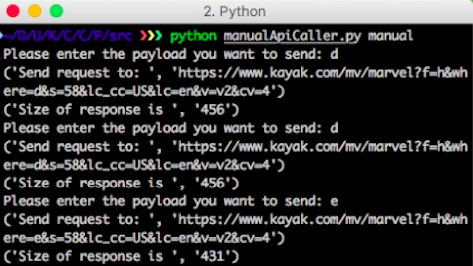
\includegraphics[width=0.48\textwidth]{images/manualApiCallerForSniffingTest.png}
\caption{The manual API Caller we used to simulate user input in the search bar}
\label{fig:manualApiCaller}
\end{figure}

\medskip

While figure \ref{fig:sniffingInference} shows successful inference, we should not forget to mention that ut tool does mistakes in the case where network traffic is hard to distinguish. In the case where payloads' traffic size are very close to one another, a slight change in the server's response (a change in a HTTP header for instance) might fool our tool and make it infer a wrong payload. However, despite such errors, our tool is working as expecting. In fact, our goal was to automate side channel leaks exploit, not to develop a perfect inference over TLS. In the case where the traffic is barely distinguishable, a "real" attacker would also have some troubles in inferring the underlying user input. For now, our results are "empirical" and based on the numerous simulations we made. We encountered some difficulties when we tried to launch our final precomputation (see Section  \ref{sect:Limitations}). We believe, however, that our tool could be extended and improved in order to make it less error prone and more accurate (see Section \ref{sect:Improvements}).


\section{Limitations}
\label{sect:Limitations}

Limitation -- Say that we need a lot of network traces to avoid the noise from the data. --> So pretty long precomputation  and many network traces to generate

-- Problems we encountered with DDOS and DigitalOcean and so on

-- Many traffic generated by the kayak web app (hard to follow and analyze)

\section{Improvements}
\label{sect:Improvements}

Explain that we did everything from scratch in this project. This took us quite a lot of time and asked us to design the entire thing. At the end of the project, we came up with possible optimization -- such as using ML algorithms and maybe neural networks to learn from the different traces of our DB and. Instead of building a 'database.json' using the mean, we could have had an intelligent Agent learning from the different traces and doing inference on the user inputs based on what it knows. Since we spend our entire time trying to design and implement our attack, we didn't have time to do it, but this would undoubtedly worth trying to go further and see whether ML techniques could improve our results.
- Since a request/response flow happens every time the user hits a keystroke, we could also use timing information and bind this information with the keyboard layout of the victim (if known, but in general we can know it pretty easily because entire regions of the world use the same keyboard layout, so if the IP address of the victim is in the US, chances are that the keyboard layout is a QWERTY US keyboard) in order to infer the keystroke that has been hit, with more accuracy (see the SSH timing attack paper)
- Database of pages fingerprints -- instead of knowing the page on which the user is in order to attack him, we could "fingerprint" a range of vulnerable websites (which means that we could see the network traffic generated when we fetched the home page of these websites, and thus, store this web trace in a DB in order to infer the page that the victim is consulting), and use these "fingerprints" to know on which pages the user is. Then, we could have a database (something like MongoDB) with many collections, each corresponding to the precomputation of a vulnerbale website, and then use this DB to swith from one collection to another as we detect that the user's browser is rendering a vulnerable page.

\section{Conclusion}

Conclude about the project:
- What we learnt from it
- How critical side channel leaks are


\section{Further research}

During our research we studied other sort of attacks that constitute real threats for our privacy on the web. The first paper we wanted to mention is called \ul{"Imperfect Forward Secrecy: How Diffie-Hellman Fails in Practice"} and has been written by a team of French and American researchers. This research put the accent on the danger to keep using export-cryptography (DHE\_EXPORT) to secure our communications. In addition of explaining their attack (Logjam) used to compute a solution of the Diffie-Hellman Problem\footnote{https://en.wikipedia.org/wiki/Diffie-Hellman\_problem} in "real time", they explained how dangerous weak keys and how misconfigurations could potentially help states decrypt our HTTPS traffic, and access our personal data. This paper has a fundamental impact since it shows the gap between cryptographers and web server administrators, and pinpoints how misunderstandings can compromise people privacy on the web.

\medskip

\ul{"Loophole: Timing Attacks on Shared Event Loops in Chrome"} by Pepe Vila et. al., published in 2017 exploit a information leak from the shared event loops in Google Chrome to infer the activity of the user on the web.


\begin{thebibliography}{1}

\bibitem{SCLeaks}
\textit{"Side-Channel Leaks in Web Applications: a Reality Today, a Challenge Tomorrow"}, 
Shuo Chen et. al, 
2010

\bibitem{trafficAnalysisSSL}
\textit{"Traffic analysis of ssl encrypted web browsing"}, 
Heyning Cheng, Heyning Cheng, and Ron Avnur,
1998. 

\bibitem{trafficAnalysisHTTPOverTLS}
\textit{"Traffic Analysis of the HTTP Protocol over TLS"},
George Danezis


\bibitem{timingSSH}
\textit{"Timing Analysis of Keystrokes and SSH Timing Attacks"},
Dawn Song, David Wagner, and Xuqing Tian,
10th USENIX Security Symposium, 
2001 

\bibitem{visitedSummer}
\textit{"I Still Know what You Visited Last Summer"},
Zachary Weinberg, 
2011


\end{thebibliography}

\ifCLASSOPTIONcaptionsoff
  \newpage
\fi

\end{document}
